\subsection{Asymptotic Resilience}
\label{sec:asymp_res}

Throughout this subsection, we will assume that $x_\ast$ is an attracting rest point of a continuously differentiable ODE. Probably the most commonly used mathematical definition of resilience,  originating in theoretical ecology \cite{pimmComplexityStabilityEcosystems1984, mayStabilityComplexityModel1974, hollingResilienceStabilityEcological1973, pimm1991balance}, represents long-term return rates to $x_{\ast}$, and is measured by (the real part of) the dominant eigenvalue at linearization. 

\begin{definition}
	\label{def:asymp}
	 Let $\textbf{A} = Df(x_\ast)$ denote the Jacobian, and recall that all eigenvalues of $\mathbf{A}$ have negative real part. Let $\lambda_1(\textbf{A})$ be the eigenvalue with largest (closest to 0) real part. 	The \textbf{asymptotic resilience} of the system at the stable rest point is equal to the negative of that real part, $$-Re(\lambda_1(\textbf{A})).$$

Note: we will refer to $\lambda_1$ as the \textbf{dominant eigenvalue} or the \textbf{slow eigenvalue} of $\mathbf{A}$. 
	 \qed 
\end{definition}

For the linearized system $x'= \textbf{A}x$, asymptotic resilience estimates the rate at which trajectories approach the equilibrium. The following theorem is standard theory for linear ODEs. %See for example (Chicone p. 175) \todo{do citation}


\begin{theorem}
	For an $n \times n$ matrix $\mathbf{A}$, if $Re(\lambda) < L < 0$ for all eigenvalues $\lambda$ of $\mathbf{A}$, then there is some constant $C>0$ such that for all $x \in \mathbb{R}^n$ and $t \geq 0$,
	%
	$$|e^{t\mathbf{A}}x| \leq Ce^{L t}|x|.$$ 
	%
	And in the long term $C$ can be taken to equal $1$. That is, there is some $T \geq 0$ such that
	%
	$$|e^{t\mathbf{A}}x| \leq e^{L t}|x| ~ ~\text{ for all } t \geq T.$$
	
	%Further, in the limit, and for all $x$ except on a set of measure 0, the inequality can be replaced with equality and $L$ can be replaced with asymptotic resilience.
	%
	%$$\lim\limits_{t \to \infty} |e^{tA}x| = e^{Re(\lambda_1) t}|x| ~ ~\text{ for almost all } x.$$ \todo{make sure this last part is true and include a proof in the appendix}
	
	 \qed
\end{theorem}


%TO DO: Is there a converse to the inequality? how to say that this is a good bound? i.e. for almost all trajectories, and in the limit as $t\to \infty$, they do eventually decay at that rate, rather than much faster than it. I feel like this is true, but I can't find a statement of it in a book. \todo{to do}

%\begin{theorem}
%	For an $n \times n$ matrix $\mathbf{A}$, if $Re(\lambda) < L < 0$ for all eigenvalues $\lambda$ of $\mathbf{A}$, then there is some constant $T>0$ such that for all $x \in \mathbb{R}^n$ and $t \geq T$,
%	
%	$$|e^{tA}x| \leq e^{L t}|x|.$$  \qed
%\end{theorem}

Note the operator $e^{t\mathbf{A}}$ in the left hand side is exactly the flow $\varphi_t$ for the linear system $x' = \mathbf{A}x$. So this theorem says that, in the long term, trajectories must decay to the origin at an exponential rate governed by the asymptotic resilience. 

%A related theorem serves as a converse of sorts, and says that the exponential bound is a good bound, so that trajectories typically do not decay significantly faster. A proof is contained in the appendix.  \todo{Is this correct? Need to work through a proof carefully. I can't find this in a book.}
%
%\begin{theorem} For almost all initial conditions $x\in U$, and in the limit as $t \to \infty$,
%	$$ |e^{tA}x| = e^{ Re(\lambda_1)t}|x|.$$ \qed
%\end{theorem}

%\begin{theorem}
%	For almost all initial conditions $x_0 \in U$, 
%	$$\lim\limits_{t \to \infty} |\varphi_t(x_0)|' = Re(\lambda_1)|\varphi_t(x_0)|,$$
%	where $' = \dfrac{d}{dt}$, and $\lambda_1$ is the dominant eigenvalue of $\mathbf{A}$.
%\end{theorem}

%\todo{write proof.}

For nonlinear systems, similar results for decay rate are justified by the Stable Manifold Theorem, a fundamental result which says that, at sufficiently nice rest points, the linear approximation is a good approximation. 
%
%The theorem states that there is a local  Moreover, the flow restricted to the stable and the unstable manifolds has exponential (hyperbolic) estimates similar to the inequalities in display (4.1)
%
%
A special case of the Stable Manifold Theorem is stated here, while a full version can be found in any standard text. %is relegated to the appendix. 

\begin{theorem}(Stable Manifold Theorem, for attracting rest points)
	Consider a non-linear system 
	%
	$$x' = \mathbf{A}(x) + h(x),$$ 
	%
	where $\mathbf{A}, h: \mathbb{R}^n \to \mathbb{R}^n$ with $\mathbf{A}$ linear.  Let $\phi_t$ be the local flow.
	%
	Assume there is an attracting rest point at the origin. 
	%
	Let $\lambda_1$ be the dominant eigenvalue of $\mathbf{A}$. Then there exists a neighborhood $N \ni 0$ which is a \textbf{local stable manifold} of the origin. 
	%
	That is, for all $x \in N$, $\lim\limits_{t \to \infty} \phi_t(x)= 0$.
	
	Furthermore, for any $Re(\lambda_1) < L < 0$, there exists $C >0$ such that for all $x \in N$, $t \geq 0$,
	%
	$$|\phi_t(x)| \leq Ce^{Lt}|x|,$$
	%
 	and for some $T \geq 0$, $C$ can be taken to equal $1$
	%
	$$|\phi_t(x)| \leq e^{L t}|x| ~ ~\text{ for } t \geq T.$$
	%Finally, in the limit, and for all $x\in N$ except on a set of measure 0, the inequality can be replaced with equality and $L$ can be replaced with asymptotic resilience.
	%
	%$$\lim\limits_{t \to \infty} \phi_t(x)| = e^{Re(\lambda_1) t}|x| ~ ~\text{ for almost all } x.$$ \todo{make sure this last part is true and include a proof in the appendix}
	\qed
\end{theorem}

%TO DO: does that last statement about long term $C=1$ hold? Can't find this in a book but I feel like it should be true. And also, what about a converse to the inequality? Does anything like that exist for the stable manifold theorem, if it does for linear systems? \todo{to do}

The theorem implies that any trajectory beginning sufficiently close to equilibrium decays toward equilibrium at an exponential rate, where that rate is determined in the long term by asymptotic resilience. Any point which is very close to, but not quite at, the equilibrium represents a state slightly perturbed away from steady state. Hence, the rate of decay can be thought of as the recovery rate from a small perturbation. 

%Hence, asymptotic resilience bounds the rate of return to equilibrium after a small perturbation to the system. Because local bifurcation is characterized by $Re(\lambda_1)$ passing through zero, the system recovers slower when nearer to bifurcation. This is the core idea of critical slowing down, which will be explained further in Section \ref{sec:csd}.

\begin{remark}
	Note that trajectories need not decay monotonically in distance to the rest point, not even for linear systems. For instance, a trajectory can initially amplify in magnitude -- a phenomenon termed \textbf{reactivity} by Neubert and Caswell in \cite{neubertAlternativesResilienceMeasuring1997} (Figure \ref{fig:reactivity}). However, with some large enough choice of $T$, the Stable Manifold Theorem still implies that short term growth negligibly affects long term decay. 
\end{remark}	

\begin{figure}[ht]
	\centering
	\captionsetup{width=0.8\linewidth}
	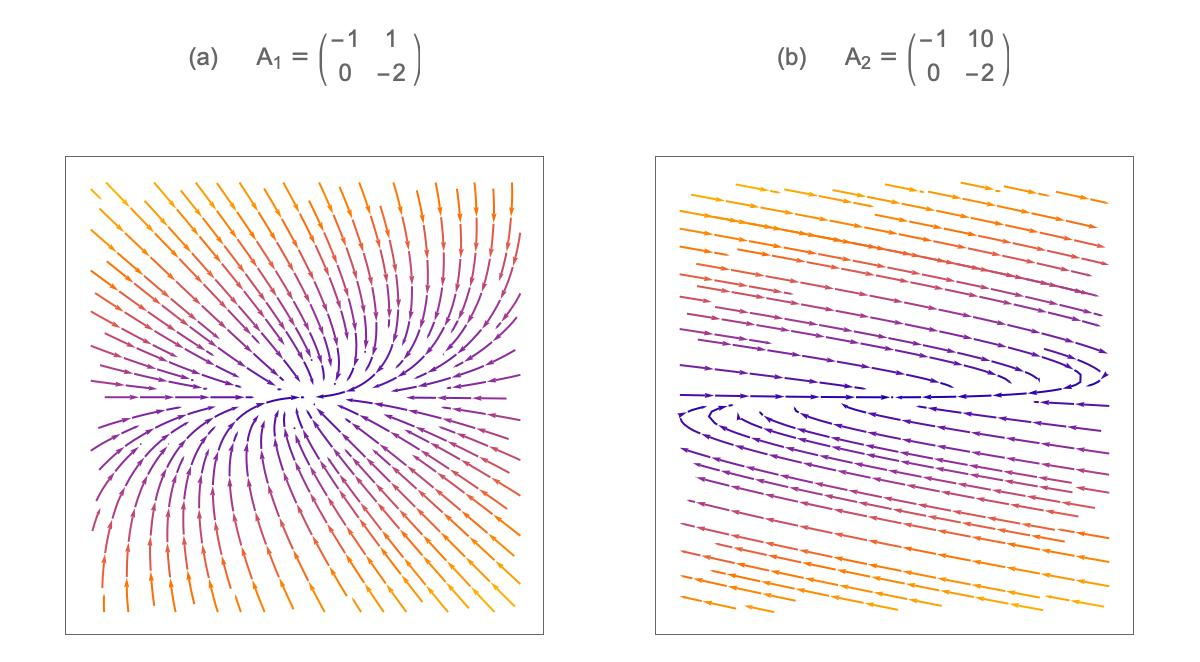
\includegraphics[width=0.8\textwidth]{figs/positive_reactivity_real_example}
	\caption{Phase portraits of two linear systems $x' = \textbf{A}x$. (a) All trajectories decay monotonically in magnitude. (b) There are trajectories beginning arbitrarily close to the origin which initially increase in magnitude. Notice that both matrices have the same eigenvalues $\lambda = -1, -2$; hence asymptotic resilience cannot tell whether an equilibrium is reactive. Example reproduced from \cite{neubertAlternativesResilienceMeasuring1997}.}
	
	\label{fig:reactivity}
\end{figure} 